\subsubsection{Accès aux prédécesseurs dans la boucle vectorisée}
La vectorisation rapproche les calculs de colonnes voisines, mais leurs dernières correspondances peuvent se trouver à des positions différentes. Pour observer ces lectures sur l’EPYC~9654, le module LProf de MAQAO~2025.1.4~\cite{maqao} échantillonne les cycles pendant seize alignements de deux préfixes homologues du chromosome~21. Chacun compte 32\,768 bases et leur distance vaut 1\,479. Sur un cœur, la boucle de mise à jour concentre 99,15\,\% des échantillons. L’analyse statique de cette boucle repère une instruction qui rassemble huit scores à des adresses calculées séparément (figure~\ref{fig:maqao-initial}).
\begin{figure}[!htbp]\centering
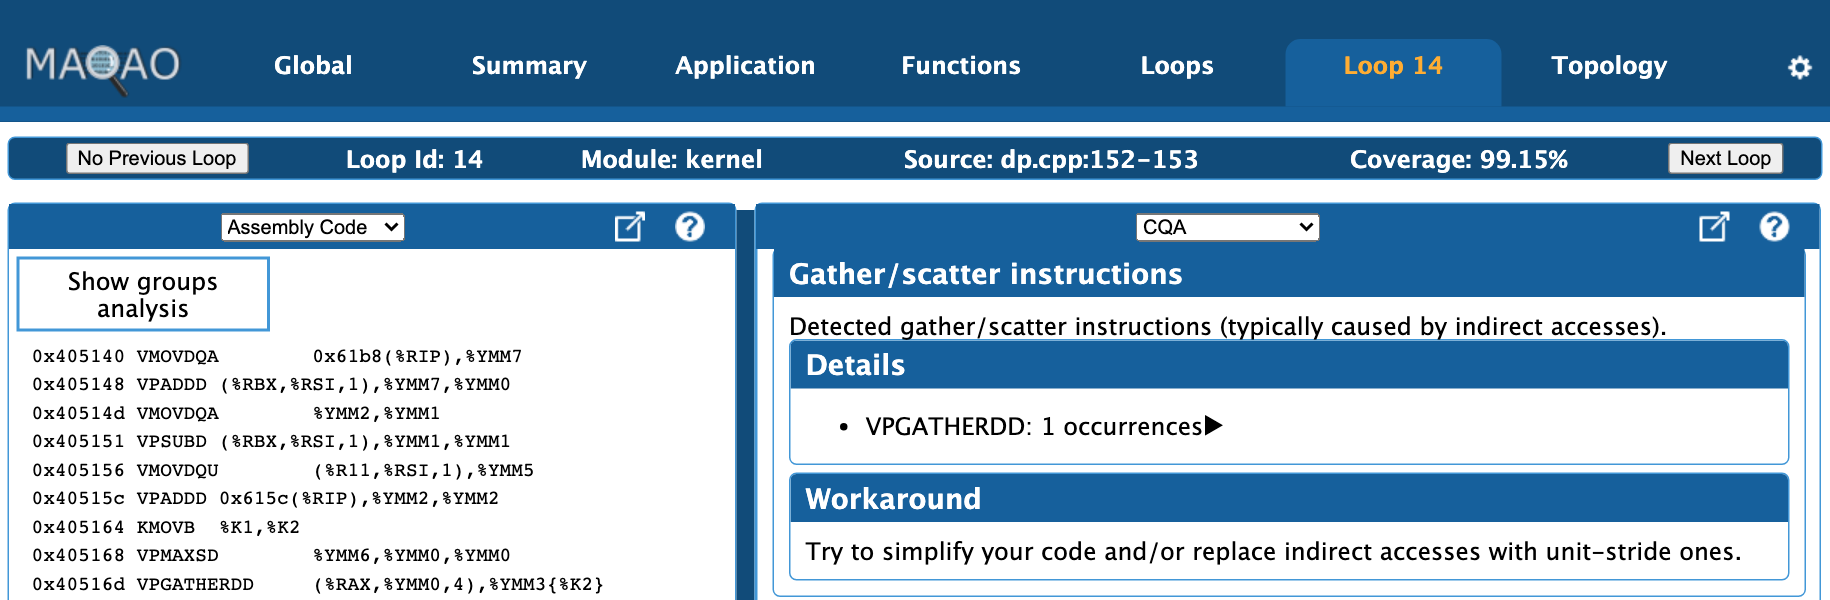
\includegraphics[width=.98\linewidth]{figures/maqao/boucle-initiale.png}
\sourcefig{bench/cpu/maqao/profile.sbatch}\caption{MAQAO affiche l’assembleur de la boucle initiale à gauche et signale à droite les lectures indirectes de l’instruction \texttt{VPGATHERDD}.}\label{fig:maqao-initial}
\end{figure}

Pour réunir ces lectures, le noyau divise chaque ligne en blocs de seize colonnes. En posant \(F_{i,j}=D_{i,j}-j\), où \(D_{i,j}\) est la distance entre préfixes, la récurrence de l’algorithme~\ref{alg:nvpd} devient, pour \(i,j\geq1\),
\[
 F_{i,j}=\min\!\left(F_{i-1,j}+1,\ F_{i-1,j-1},\ F_{i-1,k-1}-1\right).
\]
L’indice \(k\) désigne la dernière occurrence de la lettre courante jusqu’à la colonne \(j\). En son absence, la convention \(F_{i-1,-1}=i\) donne au troisième terme la valeur \(i-1\), qui majore \(D_{i,j}-j\). Les autres bords valent \(F_{0,j}=0\) et \(F_{i,0}=i\).

Par exemple, pour une ligne associée à \texttt{A} et un bloc commençant par \texttt{CCTA}, les trois premières colonnes partagent la dernière occurrence extérieure au bloc. La quatrième trouve sa correspondance dans le bloc. Une lecture scalaire fournit le score extérieur, puis une permutation en registres choisit le score de chaque colonne. Pour chaque lettre, seize indices de 32~bits occupaient 64~octets. Le bloc utilise seize indices d’un octet et une position de quatre octets, soit 20~octets. Le programme choisit cette représentation pour le score seul lorsque le processeur dispose d’AVX-512F et que la séquence la plus courte compte au moins seize bases.

La comparaison porte sur deux paires de fenêtres du chromosome~21, l’une au même locus dans deux assemblages, l’autre à des loci distincts. Le chronomètre couvre l’indexation et le calcul du score après une chauffe, depuis des séquences déjà en mémoire. Sur dix répétitions, chacune des cinq variantes occupe deux fois chaque position dans l’ordre de passage. À 32\,768 bases sur un cœur, demander à GCC des vecteurs de 512~bits sans changer les accès donne un rapport \(T_{\mathrm{initial}}/T_{\mathrm{large}}=0{,}919\) au locus homologue. Le changement de variable seul donne \(0{,}634\). Avec la permutation, le rapport atteint \(2{,}868\). Le nombre de cellules calculées reste le même pour les cinq variantes.

Dans le noyau intégré à NvPD, l’instruction \texttt{VPERMI2D} remplace le rassemblement des scores (figure~\ref{fig:maqao-permutation}). Le modèle CQA, qui suppose les données présentes dans le cache L1, passe de 21~cycles pour huit cellules à 2,67~cycles pour seize. Sur quatre cœurs, deux profils de 437 alignements au même locus attribuent respectivement 11,03 et 27,49\,\% des échantillons à l’exécution OpenMP. Le noyau accélère le calcul de chaque ligne, mais une barrière sépare toujours deux lignes successives. MAQAO signale encore la conversion des indices d’un octet en entiers, l’alignement des transferts et la possibilité de dérouler la boucle.
\begin{figure}[!htbp]\centering
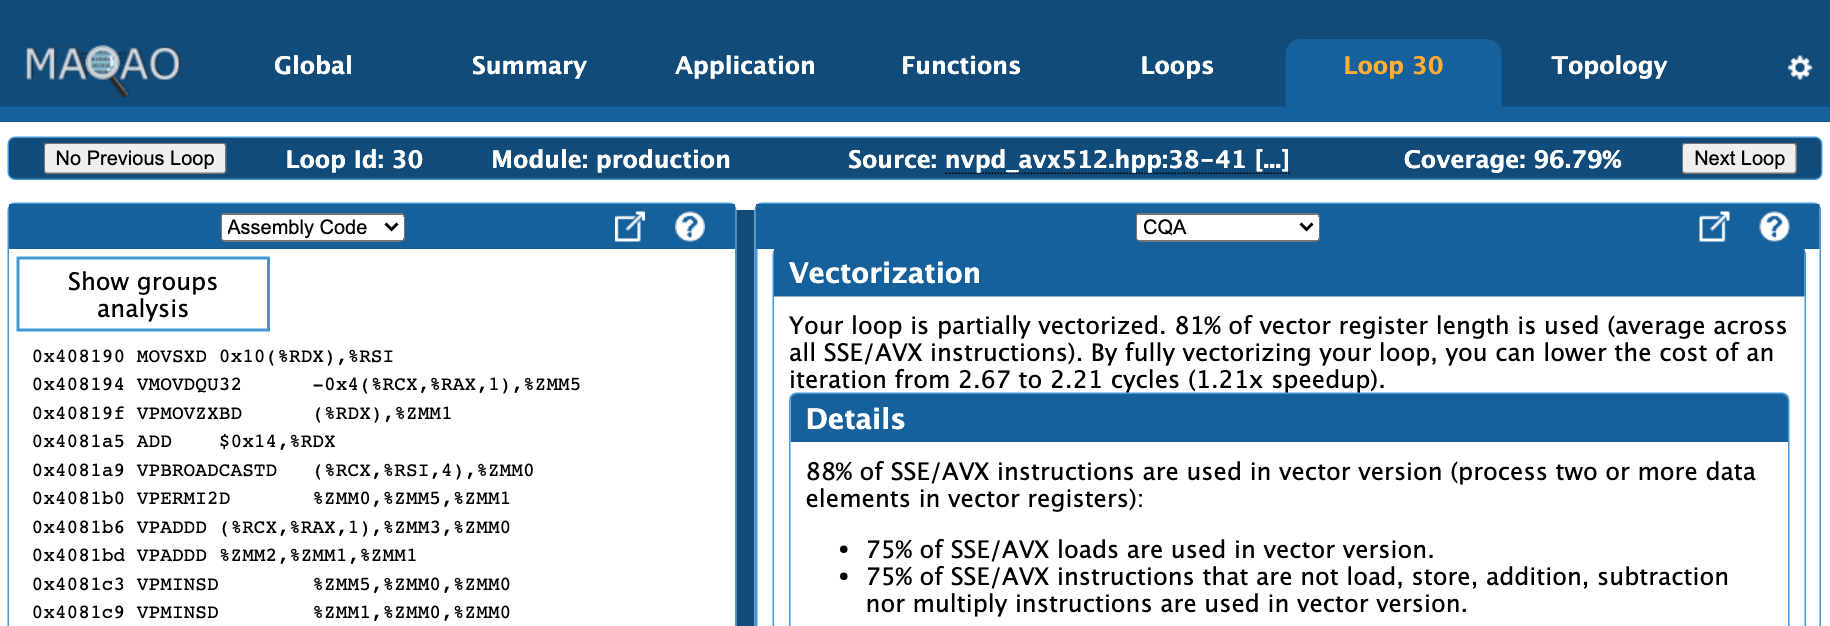
\includegraphics[width=.98\linewidth]{figures/maqao/boucle-permutation.png}
\sourcefig{bench/cpu/maqao/confirm.sbatch}\caption{Dans la boucle par blocs, la permutation réunit les prédécesseurs. Le panneau de droite estime le coût d’une itération et indique la part moyenne de la largeur vectorielle utilisée.}\label{fig:maqao-permutation}
\end{figure}

Pour vérifier si le diagnostic dépend de la version du profileur, ONEVIEW~2026.1.1 analyse sur le même nœud les deux exécutables déjà examinés avec la version~2025.1.4. À un et quatre cœurs, les 21 rapports CQA présents dans les deux séries donnent les mêmes recommandations. La version~2026.1.1 précise deux limites de la mesure. À 1\,000~Hz, LProf signale que son tampon risque de perdre des échantillons. L’avertissement disparaît à 200~Hz. À cette fréquence, ONEVIEW mesure 3,82~s pour 96 appels au noyau retenu sur quatre cœurs et 15,32~s pour 384 appels. Pour reconstruire les piles d’appels, ONEVIEW recommande de conserver le pointeur de cadre lors de la compilation.\footnote{Le pointeur de cadre aide le profileur à retrouver la fonction appelante. GCC le conserve avec \texttt{-fno-omit-frame-pointer}.} Hors du profileur, cette option allonge de 1,02\,\% le calcul au locus homologue de 32\,768 bases sur quatre cœurs (IC à 95\,\% de 0,13 à 1,92\,\%, huit blocs appariés). Dans les sept autres configurations, l’intervalle comprend zéro.

La figure~\ref{fig:maqao-temps} rapporte les gains mesurés hors du profileur. À 100\,000 bases, les deux fenêtres homologues diffèrent de 3\,345 éditions et la paire de loci distincts de 51\,331. Le nombre de cellules reste identique. Sur quatre cœurs, les permutations ramènent le temps de la paire homologue de \(1{,}0331\pm0{,}0015\) à \(0{,}2750\pm0{,}0032\)\,s (moyenne et écart-type de huit blocs).
\chart{cpu/maqao_nvpd.png}{Le gain vaut \(T_{\mathrm{initial}}/T_{\mathrm{variant}}\). À 32\,768 bases, la moyenne géométrique donne le même poids aux deux paires. À 100\,000 bases, les deux nombres sous chaque moyenne donnent l’écart-type et la demi-largeur de l’intervalle de confiance à 95\,\%.}{fig:maqao-temps}{python/studies/maqao.py}

Pour examiner les indications qui subsistent, une seconde comparaison prend le noyau par blocs comme référence (figure~\ref{fig:maqao-conseils}). Une variante aligne sur 64~octets l’écriture des scores et l’une des deux lectures contiguës. L’autre lecture est décalée d’un entier. Une deuxième variante stocke directement les seize indices sur 32~bits. Elle évite leur conversion à chaque bloc, mais leur tableau passe de 16 à 64~octets. Les deux dernières variantes déroulent respectivement deux et quatre blocs par tour de boucle.
\chart{cpu/maqao_variantes.png}{Chaque case compare une modification isolée au noyau par blocs. Le gain en gras est la moyenne géométrique de \(T_{\mathrm{block}}/T_{\mathrm{variant}}\) sur les deux paires et dix blocs. Sous le gain figurent son intervalle à 95\,\% et le facteur d’écart-type géométrique \(s_g\).}{fig:maqao-conseils}{bench/cpu/maqao/follow.sbatch}

À 32\,768 bases sur un cœur, les indices de 32~bits ramènent le rapport de temps à \(0{,}740\) (IC à 95\,\% de 0,735 à 0,746). Sur quatre cœurs, dérouler deux blocs donne \(1{,}002\) (de 0,996 à 1,008). Le modèle CQA passe alors de 2,67 cycles pour seize cellules à 5,33 cycles pour trente-deux, soit le même débit par cellule à la précision du modèle.

À 100\,000 bases, aligner les lignes apporte encore un gain sur la paire homologue, de 1,071 sur un cœur et 1,096 sur quatre. La régularité de ce gain a été examinée sur un second nœud EPYC. En alignant les lignes dès que la séquence la plus courte atteint 40\,000 bases, le rapport entre le temps du noyau par blocs et celui du candidat vaut 1,492 à 65\,519 bases sur quatre cœurs. Il tombe à 0,820 à 65\,536 bases (IC à 95\,\% de 0,775 à 0,868), puis remonte à 1,200 à 65\,553 bases. Le nombre de cellules varie de moins de 0,11\,\% entre les deux grilles extrêmes.

Un dernier essai espace les tables de symboles d’un nombre impair de lignes de cache. Sur neuf blocs, le rapport vaut encore 0,833 à 65\,536 bases (IC à 95\,\% de 0,773 à 0,898), contre 1,350 à 65\,537. Le noyau distribué conserve les indices d’un octet et un pas de \(16\lceil n/16\rceil+2\) entiers entre les lignes de scores. Sur la paire homologue de 95\,003 bases du second nœud, sa boucle à permutation concentre 98,16\,\% des échantillons sur un cœur et 86,53\,\% sur quatre. Pour une grille de \(45\,077\times90\,019\) cellules, il est 3,315 fois plus rapide que le NvPD initial sur quatre cœurs (IC à 95\,\% de 3,287 à 3,343, moyenne géométrique sur les deux paires).

\synthese{Sur les fenêtres de 131\,072 bases du second nœud, le noyau retenu calcule le score en 0,497 et 0,498\,s sur quatre cœurs. Le gain géométrique sur les deux paires vaut 3,864 (IC à 95\,\% de 3,829 à 3,899), indexation comprise.}
